% \chapter{\ifproject%
% \ifenglish Experimentation and Results\else การทดลองและผลลัพธ์\fi
% \else%
% \ifenglish System Evaluation\else การประเมินระบบ\fi
% \fi}
\chapter{
    \ifenglish Experimentation and Results\else การทดลองและผลลัพธ์\fi
}

\definecolor{eyrie}{HTML}{1E90FF}
\definecolor{marquise}{HTML}{FF6400}

% ในบทนี้จะทดสอบเกี่ยวกับการทำงานในฟังก์ชันหลักๆ

\section{Experiment setup}

\subsection{Introductory experiment}
For the introductory experiment, Random agent is used as it has the most basic implementation. The experiments will be conducted by simulating \RootOurs \ with random actions option turned on, and collect the results. 

We will run 100,000 \glspl{playout} using a random decision agent as each faction and collect the following statistics:
\begin{itemize}
    \item winning faction: \Marquise{} / \Eyrie
    \item winning condition: 30 victory points (vp)
    \item number of turns played (the number of birdsong phase played)
    \item whose turn was it when the game ends: \Marquise{} / \Eyrie
    \item victory points of \Marquise{} when the game ends
    \item victory points of \Eyrie{} when the game ends
\end{itemize}

\subsection{Main experiment}
The main experiment will be conducted on multiple variants of MCTS agent to find the ``best MCTS variant'' for each faction. This experiment consists of two phases. 

\subsubsection{Setup} \label{main-exp-setup}
The base agent is an MCTS agent. It was used to play against the Random agent. The result shows that both \Marquise{} and \Eyrie{}, with base agent, are able to consistently win most of the rounds against the Random agent. This means that the Random agent cannot be used as a base since all MCTS agents would likely have very high win rate.

%TODO: result of base agent and random agent

The base agent's MCTS parameters are as follows:
\begin{enumerate}
    \item \textbf{\texttt{reward-function}}: \texttt{vp-difference}
    \item \textbf{\texttt{expand-count}}: 100
    \item \textbf{\texttt{rollout-no}}: 1
    \item \textbf{\texttt{time-limit}}: -1
    \item \textbf{\texttt{action-count-limit}}: 20
    \item \textbf{\texttt{best-action-policy}}: \texttt{robust}
\end{enumerate}

The main experiment's MCTS variants are permutations of these parameters:
\begin{enumerate}
    \item \textbf{\texttt{reward-function}}: \texttt{win}, \texttt{vp-difference}, \texttt{vp-difference-relu} (\texttt{vp-difference-bin} is excluded because it is the same as \texttt{vp-difference-relu} but is unable to separate a ``very good'' rollout from a ``good'' rollout.)
    \item \textbf{\texttt{expand-count}}: 50, 100, 200
    \item \textbf{\texttt{rollout-no}}: 1 (fixed to 1 because nondeterminism is eliminated in simulation by using \textit{determinization} as described in \ref{handling-uncertainty})
    \item \textbf{\texttt{time-limit}}: -1 (means no time limit. because the rollout time are so fast that the time limit is ignorable)
    \item \textbf{\texttt{action-count-limit}}: 20, 100, 200, -1 (-1 means no limit)
    \item \textbf{\texttt{best-action-policy}}: \texttt{max}, \texttt{robust}, \texttt{secure}
    % TODO: why is UCB removed?
    % TODO: recheck the reasons for these param choices
\end{enumerate}
These parameters resulted in 108 variants for each faction.

\subsubsection{Phase 1}
For the first phase, as there are 108 MCTS variants and 2 factions, there will be 216 battles in this phase. Each battle will be run for 100 rounds to minimize random deviation.

\subsubsection{Phase 2}
For the second phase, the top variants from the first phase will be selected to continue in this phase. The metrics of selection is ``win rate'' against the base variant. Unless some variant achieved 100\% win rate (win all 100 rounds), it is unlikely that the variants will have overlapping win rates, though if that were to be the case, other metrics will be used such as ``average turns to win'', etc. The top 5 variants for each faction will be selected. Then they all play against each of the other faction's, i.e., a ``Team Round-Robin''. There will be 25 battles in this phase. Each battle will be run for 100 rounds.

\subsubsection{Final}
Finally, the best performing variant from each faction will be selected to be the ``best MCTS variant'' for that faction.



\section{Results}

\subsection{Introductory experiment's results}

Figure \ref{fig:introductory-win} indicates that the Marquise random agent outperformed the Eyrie random agent. This result proves our assumption that the Marquise faction has a low-complexity, no-penalty gameplay mechanism that makes it easier to score a victory point than the Eyrie faction does. This corresponds to the fact that the mean victory point of the Marquise when losing is higher than that of Eyrie, as shown in Figure \ref{fig:introductory-loser-vp-dist}.

Figure \ref{fig:introductory-winner-turn-dist} shows that the average number of turns to win for Marquise and Eyrie is 30.453 and 30.252, respectively. This result can be used as the baseline performance of the AI model.

\begin{figure}[h!]
    \begin{center}
      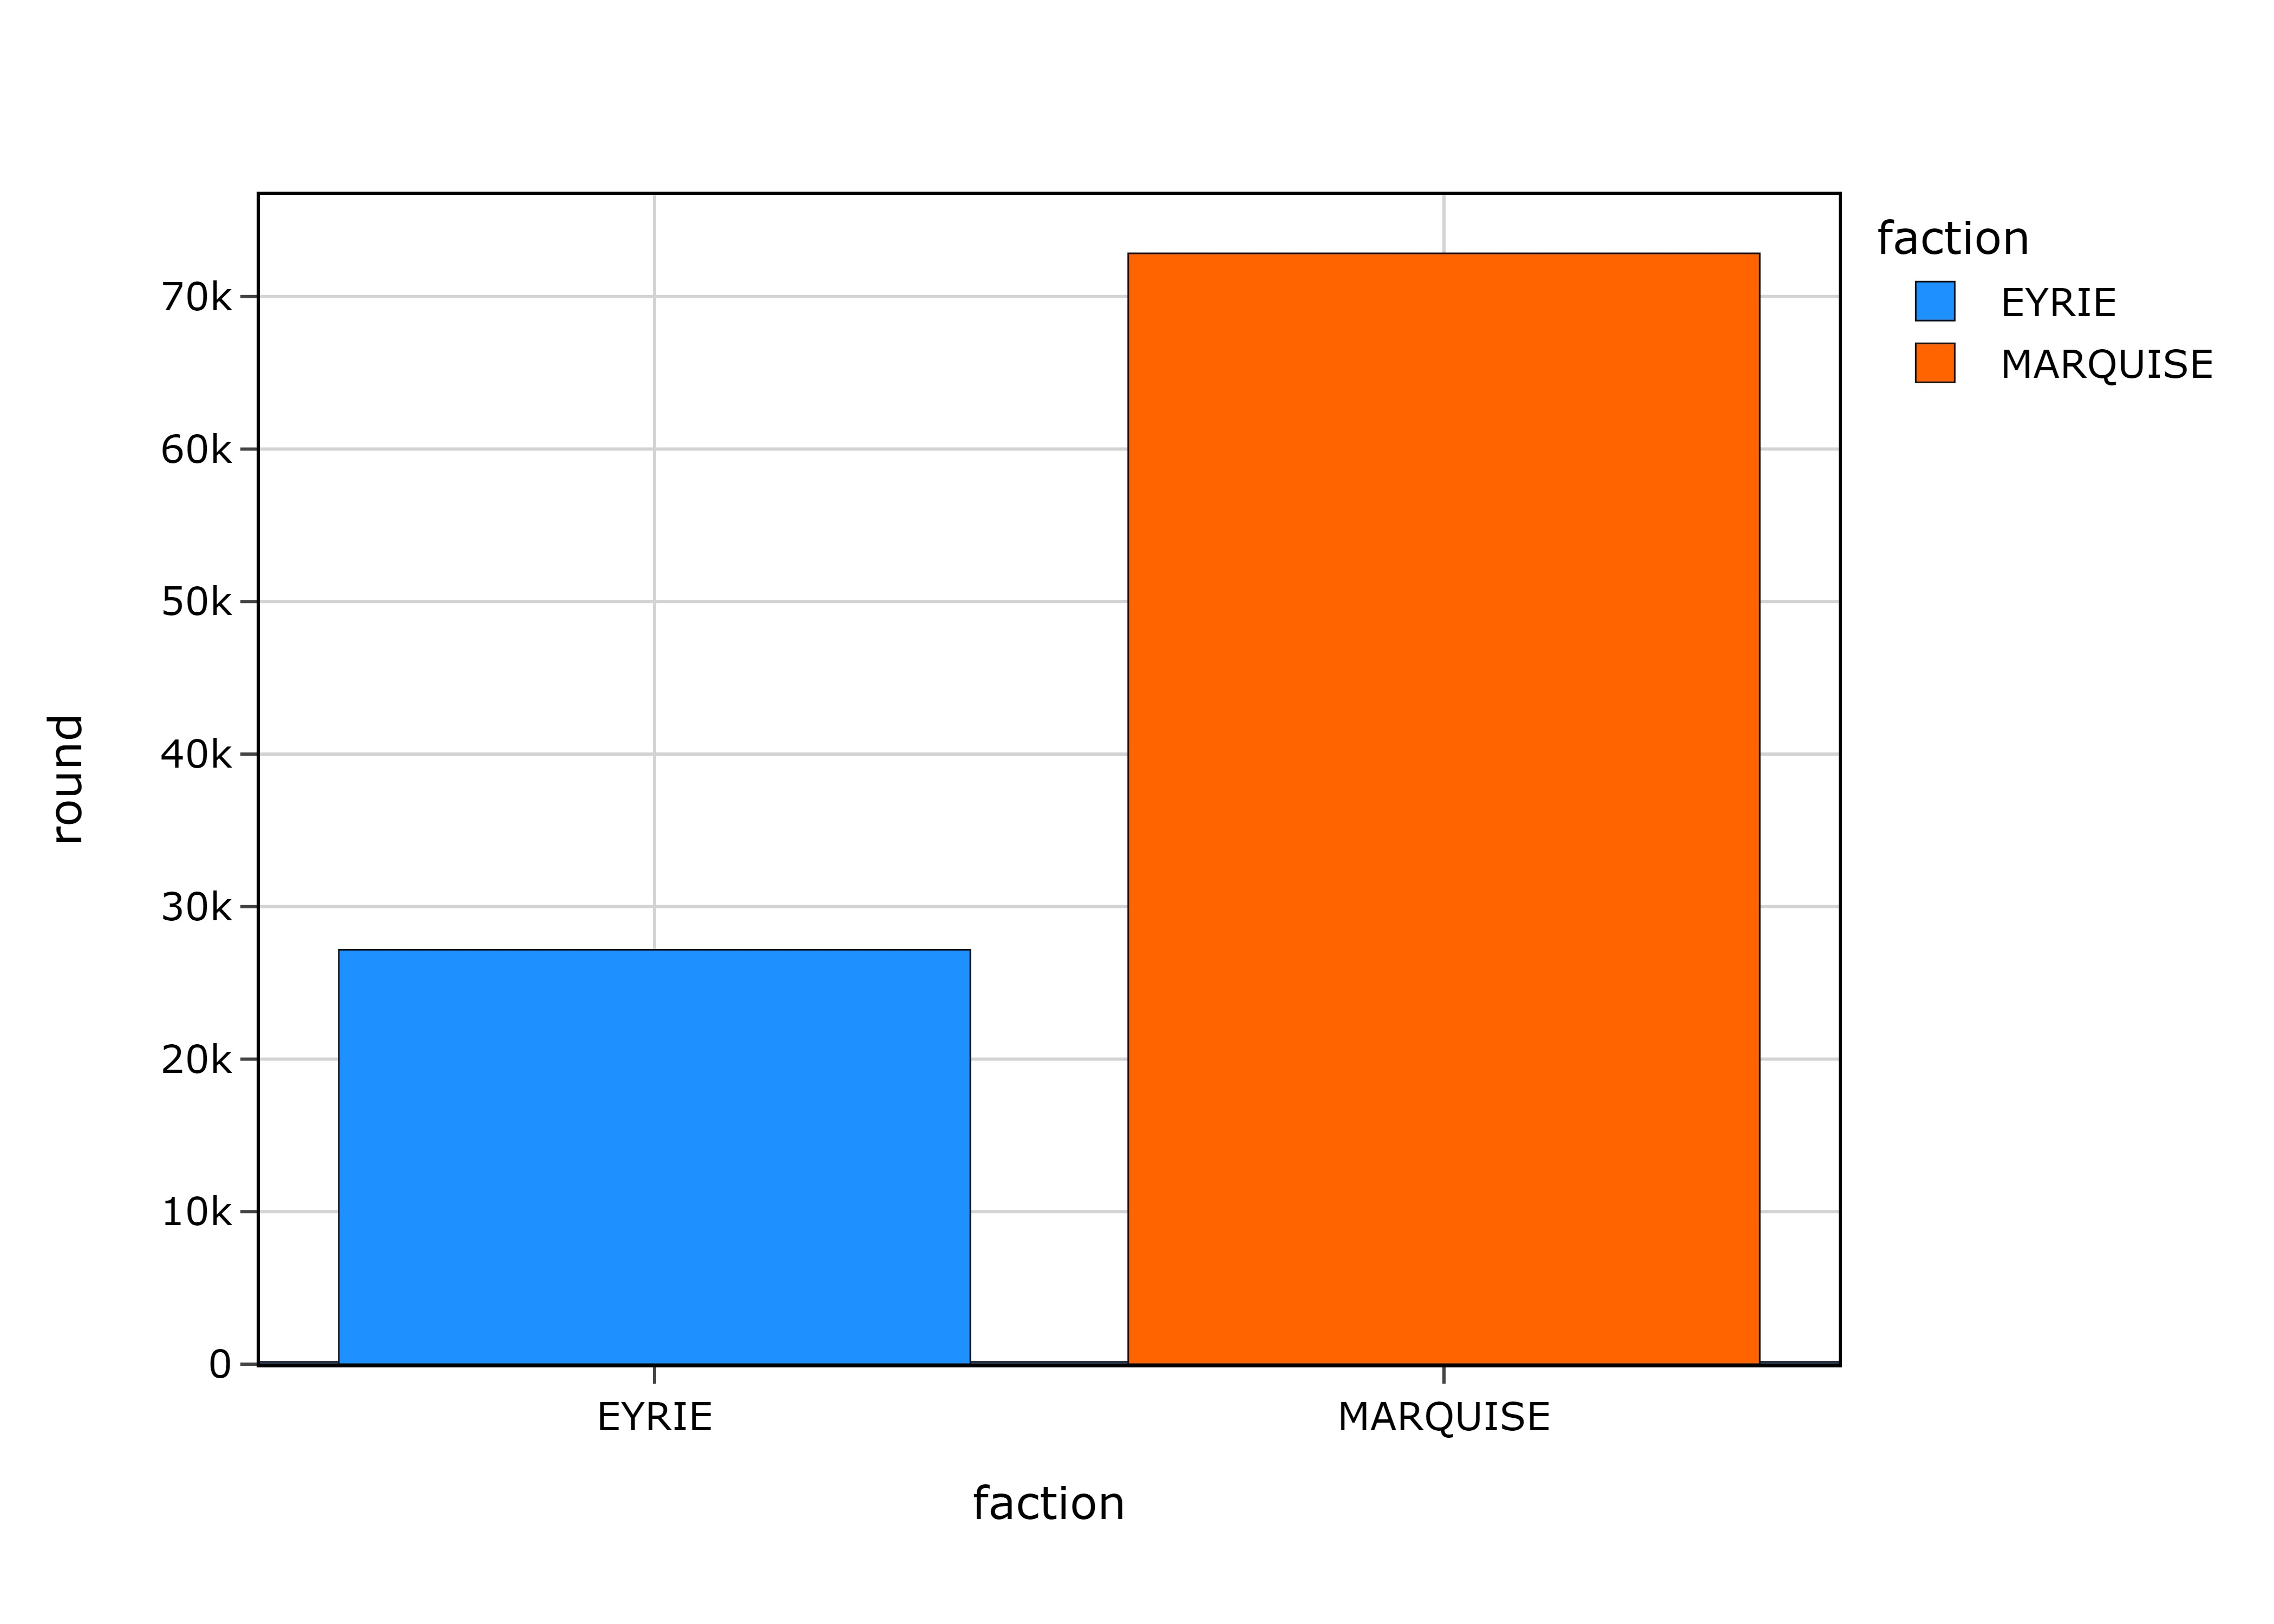
\includegraphics[width=0.9\textwidth]{./images/fig-introductory-win.jpeg}
    \end{center}
    \caption{The number of wins of each faction}
    \label{fig:introductory-win}
\end{figure}

\begin{figure}[h!]
    \begin{center}
      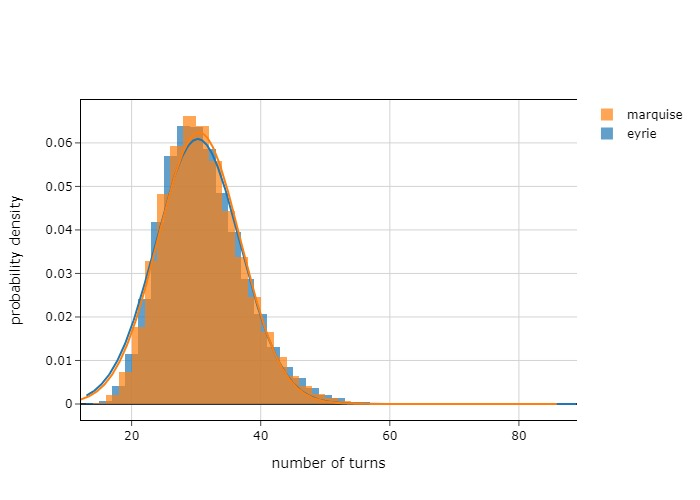
\includegraphics[width=0.9\textwidth]{./images/fig-introductory-winner-turn-dist.jpeg}
    \end{center}
    \caption{The distribution of the number of turns to win for each faction}
    \label{fig:introductory-winner-turn-dist}
\end{figure}

\begin{figure}[h!]
    \begin{center}
      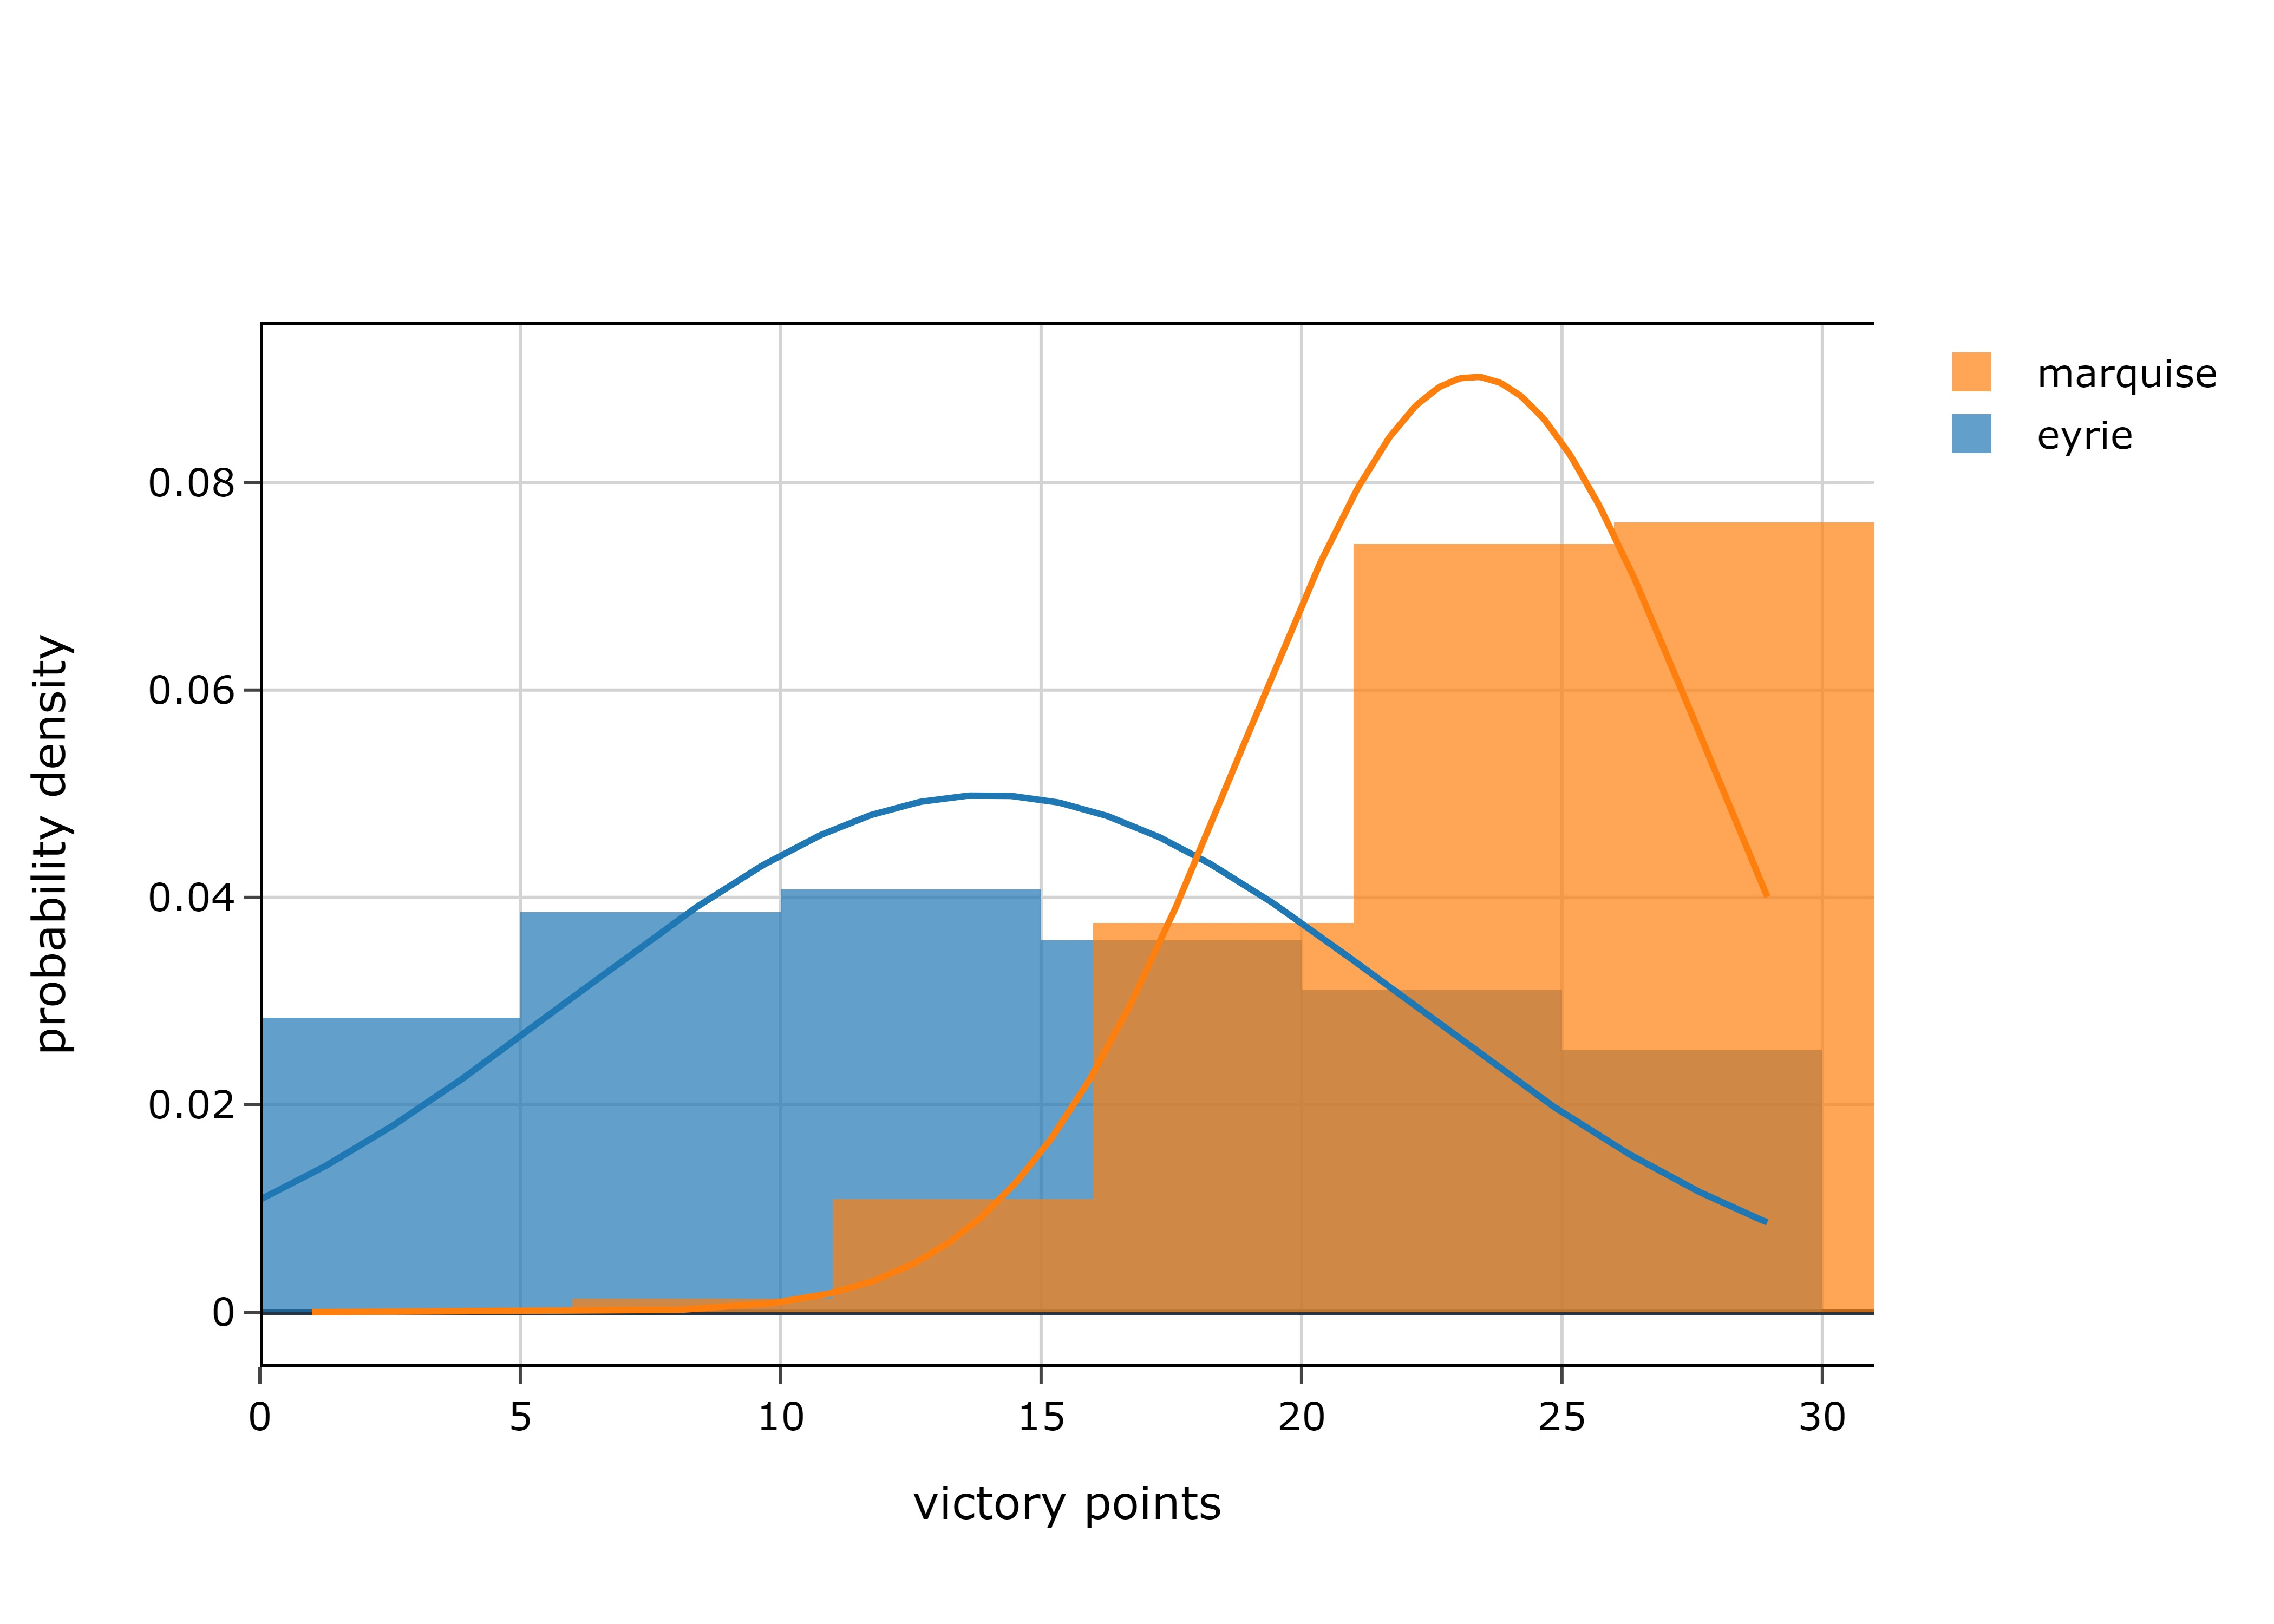
\includegraphics[width=\textwidth]{./images/fig-introductory-loser-vp-dist.jpeg}
    \end{center}
    \caption{The distribution of victory points for each faction when losing}
    \label{fig:introductory-loser-vp-dist}
\end{figure}

\subsection{Main experiment's result}

\subsubsection{Phase 1}

% \textbf{Top 5 Variants}

In this section, parameters \texttt{rollout-no} and \texttt{time-limit} are not displayed in the tables as they are fixed to 1 and -1 (no-limit), respectively.

The results of top 5 MCTS variants for \Marquise{} and \Eyrie{} versus the base variant are displayed in Table \ref{tab:mar-top5} and \ref{tab:ey-top5}

\begin{table}[h!]
    \caption{\Marquise{}'s top 5 MCTS variants versus the base variant}
    \label{tab:mar-top5}
    \centering
    \begin{tabular}{| c || P{1.2cm} | P{1.2cm} || P{4cm} | P{1.2cm} | P{1.2cm} | P{1.2cm} |} 
        \hline
        \bf config no. & \bf  win rate & \bf average match length & \bf reward function & \bf expand count & \bf action count limit & \bf best action policy \\ [0.5ex] \hline 
        86 & 0.61 & 16.787 & \texttt{vp-difference} & 200 & 100 & secure \\ \hline 
        76 & 0.55 & 15.418 & \texttt{vp-difference} & 200 & 20 & robust \\ \hline 
        85 & 0.53 & 15.547 & \texttt{vp-difference} & 200 & 100 & max \\ \hline 
        87 & 0.53 & 16.245 & \texttt{vp-difference-relu} & 200 & 100 & max \\ \hline 
        89 & 0.52 & 15.327 & \texttt{vp-difference-relu} & 200 & 100 & secure \\ \hline %[1ex] 
        \hline
    \end{tabular}
\end{table}

\begin{table}[h!]
    \caption{\Eyrie{}'s top 5 MCTS variants versus the base variant}
    \label{tab:ey-top5}
    \centering
    \begin{tabular}{| c || P{1.2cm} | P{1.2cm} || P{4cm} | P{1.2cm} | P{1.2cm} | P{1.2cm} |} 
        \hline
        \bf config no. & \bf  win rate & \bf average match length & \bf reward function & \bf expand count & \bf action count limit & \bf best action policy \\ [0.5ex] \hline 
        184 & 0.81 & 14.519 & \texttt{vp-difference} & 200 & 20 & robust \\ \hline 
        203 & 0.72 & 15.722 & \texttt{vp-difference} & 200 & 200 & secure \\ \hline 
        194 & 0.71 & 15.690 & \texttt{vp-difference} & 200 & 100 & secure \\ \hline 
        212 & 0.71 & 16.676 & \texttt{vp-difference} & 200 & -1 & secure \\ \hline 
        202 & 0.71 & 16.803 & \texttt{vp-difference} & 200 & 200 & robust \\ \hline %[1ex] 
        \hline
    \end{tabular}
\end{table}

% \textbf{Observation: Imbalance in Potential}

\Marquise{}'s win rate ranges from 0.52 to 0.61, while \Eyrie's ranges from 0.71 to 0.81. We speculated that this was due to the difference in ``potential'' between the two factions. \Marquise{}'s playstyle is straight forward because of the fixed action count per turn, while \Eyrie{} has the Decree, which dictates what actions the \Eyrie{} player can perform. The Decree, when built and followed properly, can grant the \Eyrie{} player over twice the action count per turn when compared to \Marquise{}, which grants more potential to earn VPs while also punishing with lose of VPs if played incorrectly.

% \textbf{Observation: Impact of each parameters}
Speculation on the impact of each parameters:
\begin{itemize}
    \item Most variant has \texttt{vp-difference}-based reward function. We speculated that this is due to the \texttt{win} option only working if the simulation step reaches a game-ending state and \texttt{vp-difference-relu} option not being able to differentiate a bad action from a very bad action.
    \item Every variant has expand count of 200. We speculated that if the MCTS is able to look forward further into the future and see more possible outcomes, it can then select better paths.
    \item The action count limit of 100 is the majority for \Marquise{} while \Eyrie{} has a varying action count limit. We speculated that the action count limit does not necessarily need to be high, but it needs to be at the right value that represents the outcome of a series of actions from the root state.
    \item The best action policy also varies between variants. We speculated that each option for this parameter in itself does not impact much, but if combined with fitting options for other parameters, it can then shine.
\end{itemize}

\subsubsection{Phase 2}

% \textbf{Top 1 Variants}

In this section, parameters \texttt{rollout-no} and \texttt{time-limit} are not displayed in the tables as they are fixed to 1 and -1 (no-limit), respectively.

The results of top 5 MCTS variants for \Marquise{} and \Eyrie{} versus the other faction's top 5 MCTS variants are displayed in Table \ref{tab:mar-team-rr} and \ref{tab:ey-team-rr}. The variant with highest win rate in each faction is highlighted in bold.

\begin{table}[h!]
    \caption{\Marquise{}'s top 5 MCTS variants versus \Eyrie{}'s top 5 MCTS variants}
    \label{tab:mar-team-rr}
    \centering
    \begin{tabular}{| c || P{1.2cm} | P{1.2cm} || P{4cm} | P{1.2cm} | P{1.2cm} | P{1.2cm} |} 
        \hline
        \bf config no. & \bf  win rate & \bf average match length & \bf reward function & \bf expand count & \bf action count limit & \bf best action policy \\ [0.5ex] \hline 
        86 & 0.532 & 15.363 & \texttt{vp-difference} & 200 & 100 & secure \\ \hline 
        76 & 0.390 & 15.727 & \texttt{vp-difference} & 200 & 20 & robust \\ \hline 
        \bf 85 & \bf 0.560 & \bf 15.389 & \bf \texttt{vp-difference} & \bf 200 & \bf 100 & \bf max \\ \hline 
        87 & 0.422 & 15.250 & \texttt{vp-difference-relu} & 200 & 100 & max \\ \hline 
        89 & 0.374 & 15.230 & \texttt{vp-difference-relu} & 200 & 100 & secure \\ \hline %[1ex] 
        \hline
    \end{tabular}
\end{table}

\begin{table}[h!]
    \caption{\Eyrie{}'s top 5 MCTS variants versus \Marquise{}'s top 5 MCTS variants}
    \label{tab:ey-team-rr}
    \centering
    \begin{tabular}{| c || P{1.2cm} | P{1.2cm} || P{4cm} | P{1.2cm} | P{1.2cm} | P{1.2cm} |} 
        \hline
        \bf config no. & \bf  win rate & \bf average match length & \bf reward function & \bf expand count & \bf action count limit & \bf best action policy \\ [0.5ex] \hline 
        \bf 184 & \bf 0.634 & \bf 13.681 & \bf \texttt{vp-difference} & \bf 200 & \bf 20 & \bf robust \\ \hline 
        203 & 0.520 & 15.388 & \texttt{vp-difference} & 200 & 200 & secure \\ \hline 
        194 & 0.580 & 15.217 & \texttt{vp-difference} & 200 & 100 & secure \\ \hline 
        212 & 0.450 & 15.735 & \texttt{vp-difference} & 200 & -1 & secure \\ \hline 
        202 & 0.538 & 15.517 & \texttt{vp-difference} & 200 & 200 & robust \\ \hline %[1ex] 
        \hline
    \end{tabular}
\end{table}

The variant with the highest win rate versus the other faction's top 5 MCTS variants for \Marquise{} is config number 85 with 0.560 win rate and 15.389 average match length. \Eyrie{}'s is config number 184 with 0.634 win rate and 13.681 average match length.

With the result of the best variants, we speculated that the \texttt{vp-difference} reward function is the best since it can fully represent both negative, positive, and neutral outcomes. The expand count of 200, which is highest amongs our setups, directly impacts the intelligence of the MCTS algorithm, but if it is too high, it will take too long to compute. The action count limit: for \Marquise{}, certain actions will show significant result after a while, such as building sawmills — you will get wood in later turns instead of the turn you build it. But for \Eyrie{}, every card added to the Decree will be effective immediately and every action will impact the close-future of that turn (and also far-future); A wrong action will quickly lead to a Turmoil for the Eyrie player. As for best action policies, we still cannot explain why \texttt{max} and \texttt{robust} are performing best for each faction, or if they has significant impact to the algorithm at all.

\begin{figure}[h!]
    \begin{center}
      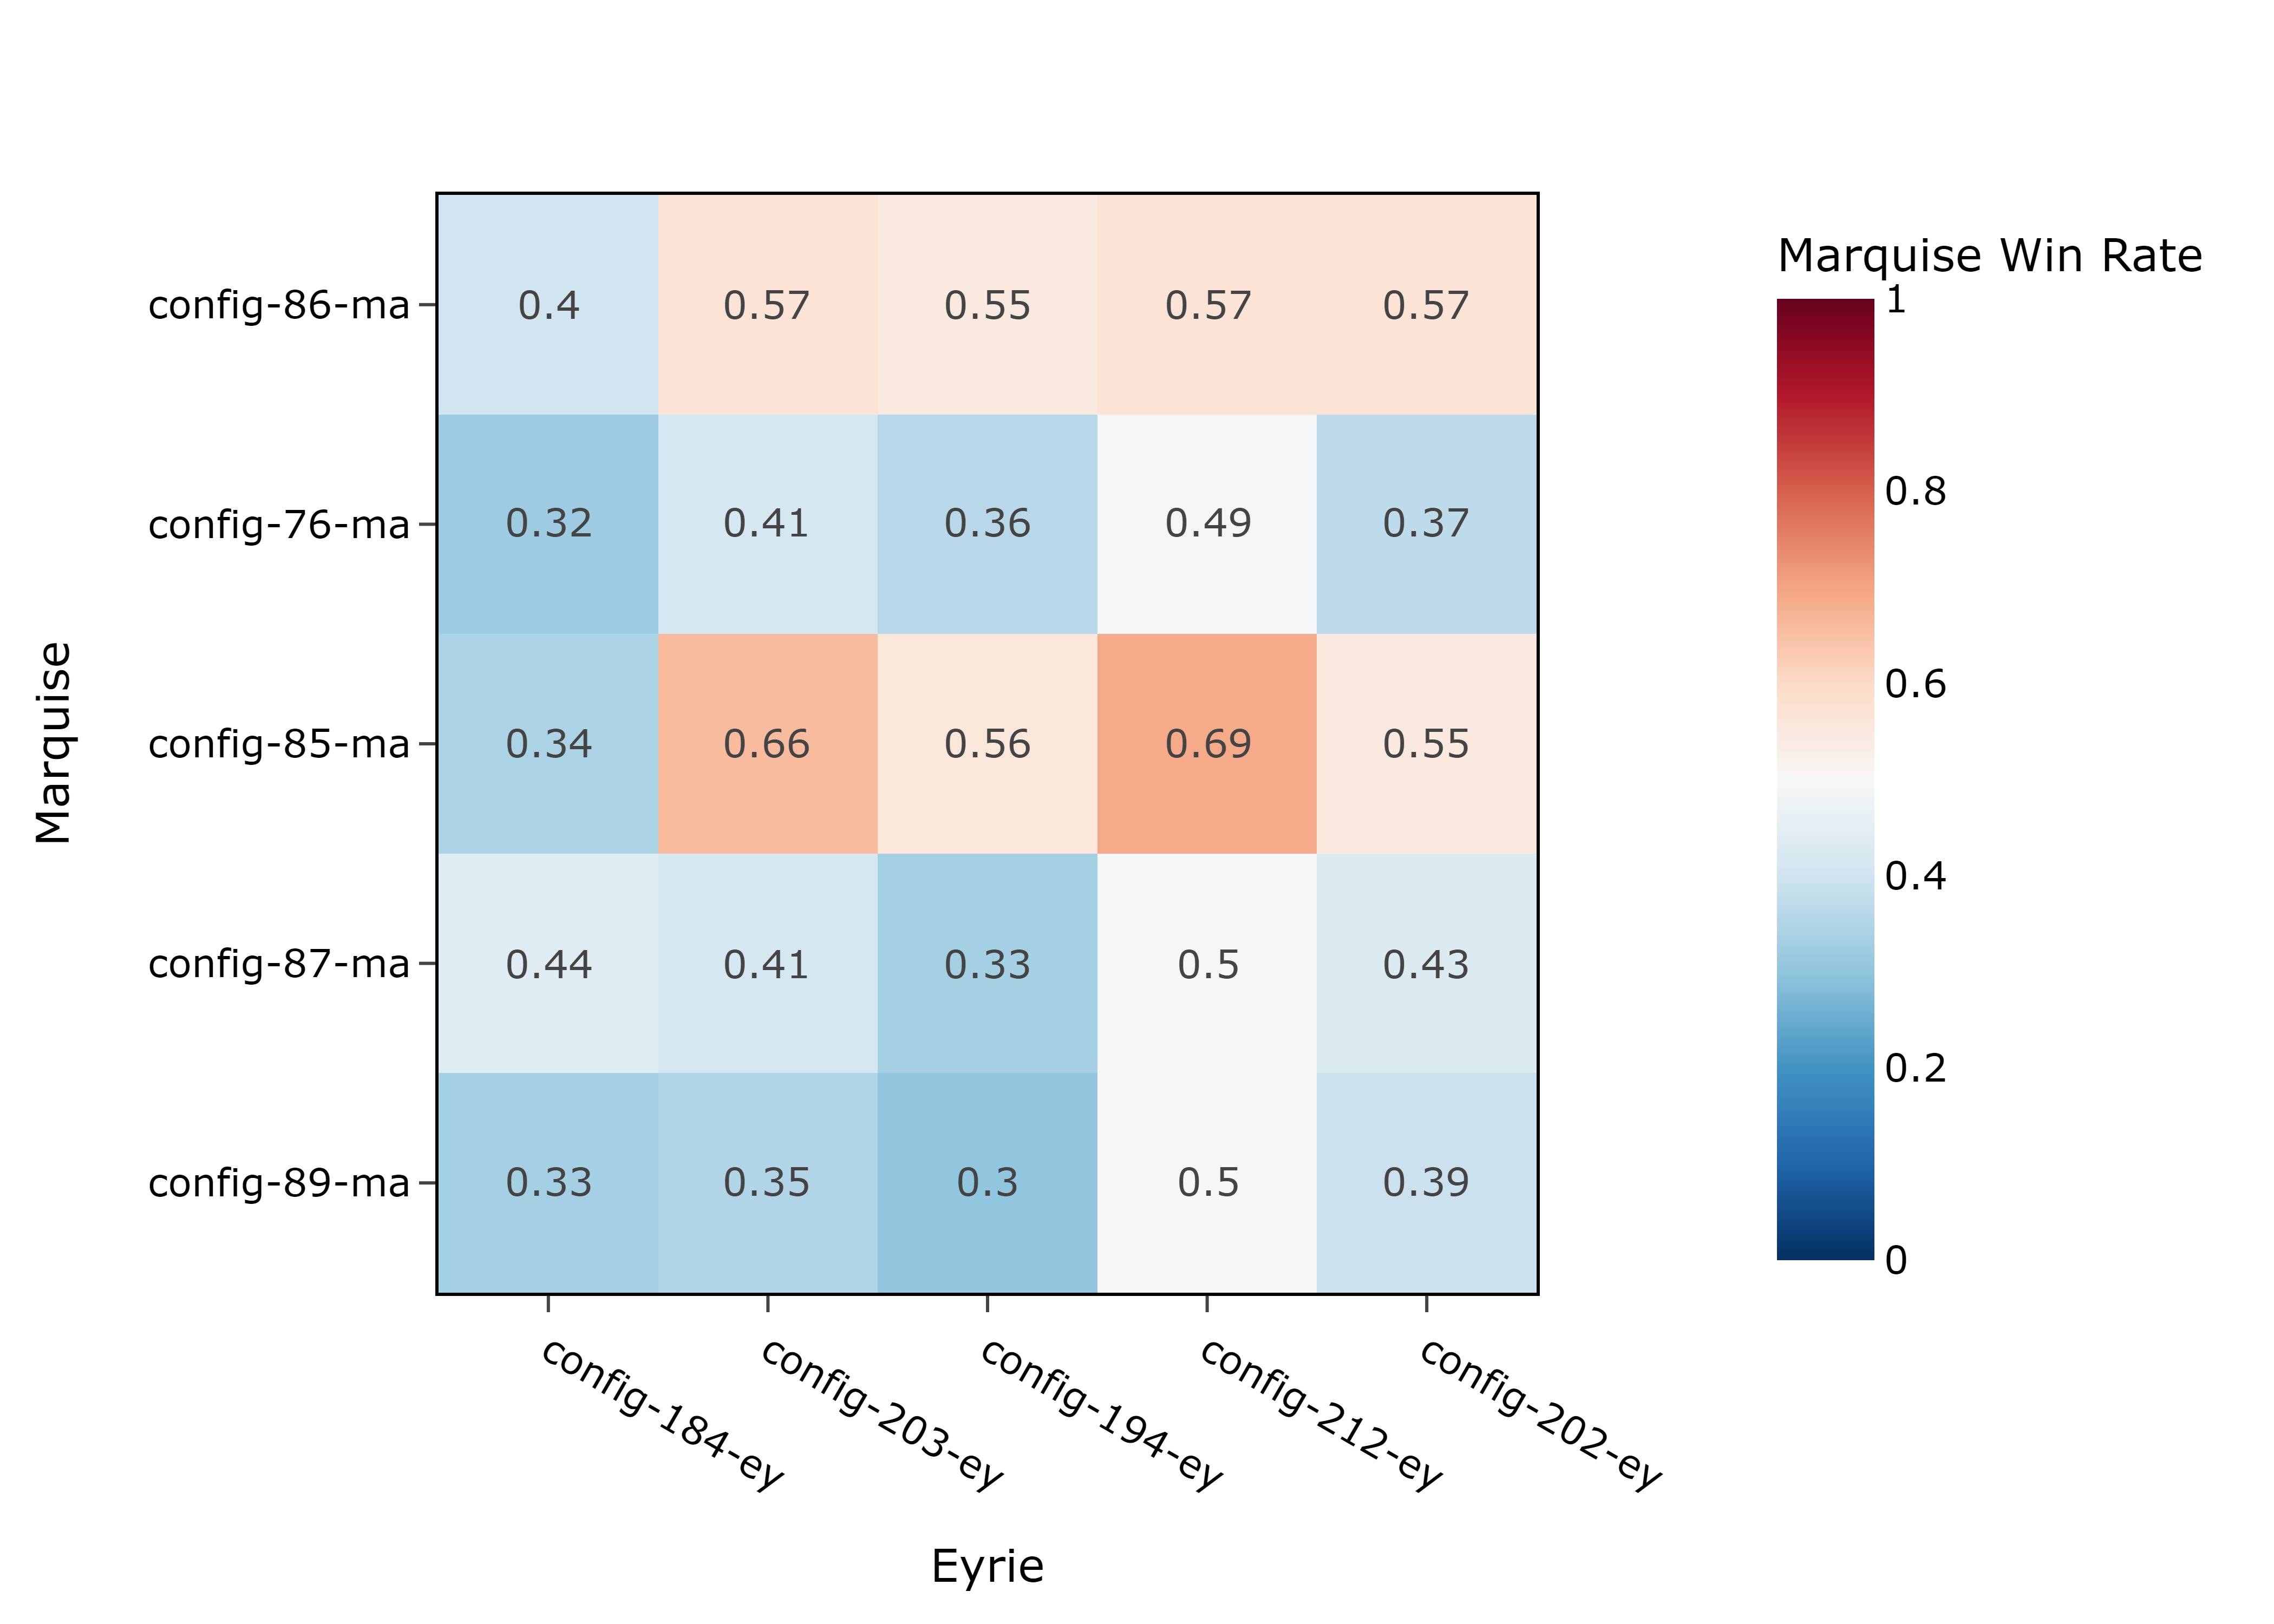
\includegraphics[width=\textwidth]{./images/fig-stage-2-marquise-win-rate.jpeg}
    \end{center}
    \caption{Top 5 Marquise variants win rate againts top 5 Eyrie variants: individual battle}
    \label{fig:top-5-ma-wr-against-top-5-ey}
\end{figure}

\begin{figure}[h!]
    \begin{center}
        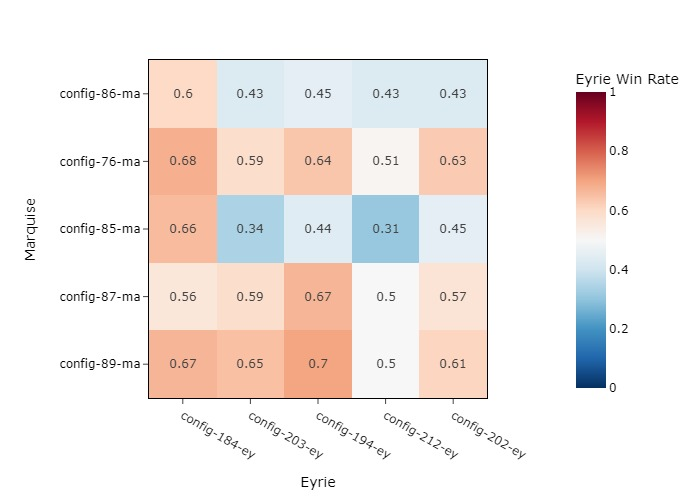
\includegraphics[width=\textwidth]{./images/fig-stage-2-eyrie-win-rate.jpeg}
    \end{center}
    \caption{Top 5 Eyrie variants win rate againts top 5 Marquise variants: individual battle}
    \label{fig:top-5-ey-wr-against-top-5-ma}
\end{figure}

The win rate for \Marquise{} seems low, but if looking at each individual battle in Figure \ref{fig:top-5-ma-wr-against-top-5-ey}, the result show that config 86 and 85 performed well; having won all \Eyrie{}'s configs except for config 184. In contrast to \Eyrie{} in Figure \ref{fig:top-5-ey-wr-against-top-5-ma}, only config 184 won all \Marquise{}'s configs while others lost to config 86 and 85.

% TODO: add result graph